% !TeX root = ../../Skript.tex
\cohead{\Large\textbf{Monotonie}}
\fakesubsection{Monotonie}
Die Begriffe positive/negative Steigung bzw. steigende/fallende Funktion haben wir bereits intuitiv verwendet. Jetzt wollen wir diese mathematisch definieren.
\begin{tcolorbox}
	Monoton wachsende Funktionen:

	\textcolor{loestc}{Eine Funktion \(f(x)\) ist monoton wachsend, wenn die Funktionswerte mit steigenden x-Werten größer werden.}

    \bigskip

\end{tcolorbox}
\begin{minipage}{\textwidth}
	\adjustbox{valign=t}{\begin{minipage}{0.6\textwidth}
		Beispiel: \(f(x)=\frac{1}{10}x^3\)

		\textcolor{loes}{Aus \(x_1\leq x_2\) folgt \(f(x_1 )\leq f(x_2)\)}

		\textcolor{loes}{Diese Funktion ist auf ganz \(\R\) monoton wachsend.}

		\textcolor{loes}{Beim Zeichnen des Schaubilds der Funktion muss man mit dem Stift immer weiter nach oben gehen.}
	\end{minipage}}%
	\adjustbox{valign=t, padding=2ex 0ex 0ex 0ex}{\begin{minipage}{0.4\textwidth-2ex}
		\centering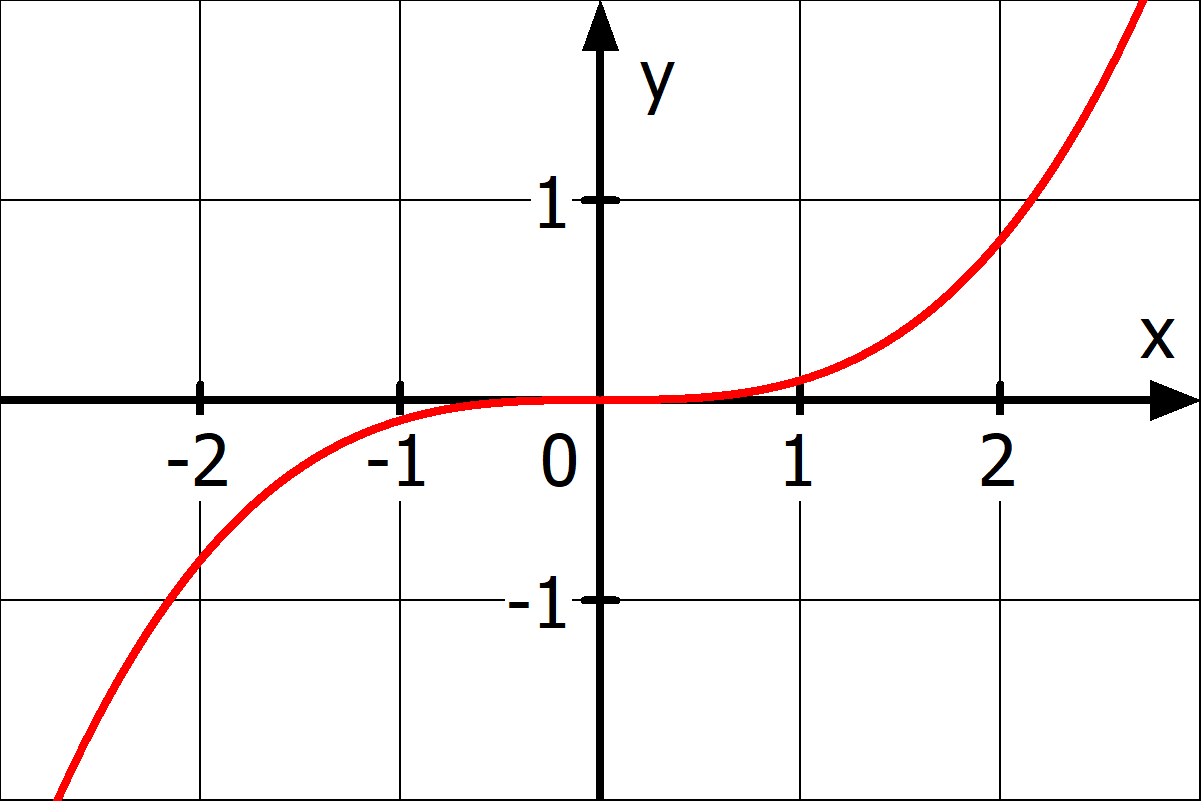
\includegraphics[width=\textwidth]{\ableitung/pics/monotonieBsp1.png}
	\end{minipage}}%
\end{minipage}

\begin{tcolorbox}
	Monoton fallende Funktionen:

	\textcolor{loestc}{Eine Funktion \(f(x)\) ist monoton fallend, wenn die Funktionswerte mit steigenden x-Werten kleiner werden.}

    \bigskip

\end{tcolorbox}
\begin{minipage}{\textwidth}
	\adjustbox{valign=t}{\begin{minipage}{0.6\textwidth}
		Beispiel: \(f(x)=e^{-x}-1\)

		\textcolor{loes}{Aus \(x_1\leq x_2\) folgt \(f(x_1 )\geq f(x_2)\)}

		\textcolor{loes}{Diese Funktion ist auf ganz \(\R\) monoton fallend.}

        \textcolor{loes}{Beim Zeichnen des Schaubilds der Funktion muss man mit dem Stift immer weiter nach unten gehen.}
	\end{minipage}}%
    \adjustbox{valign=t, padding=2ex 0ex 0ex 0ex}{\begin{minipage}{0.4\textwidth-2ex}
		\centering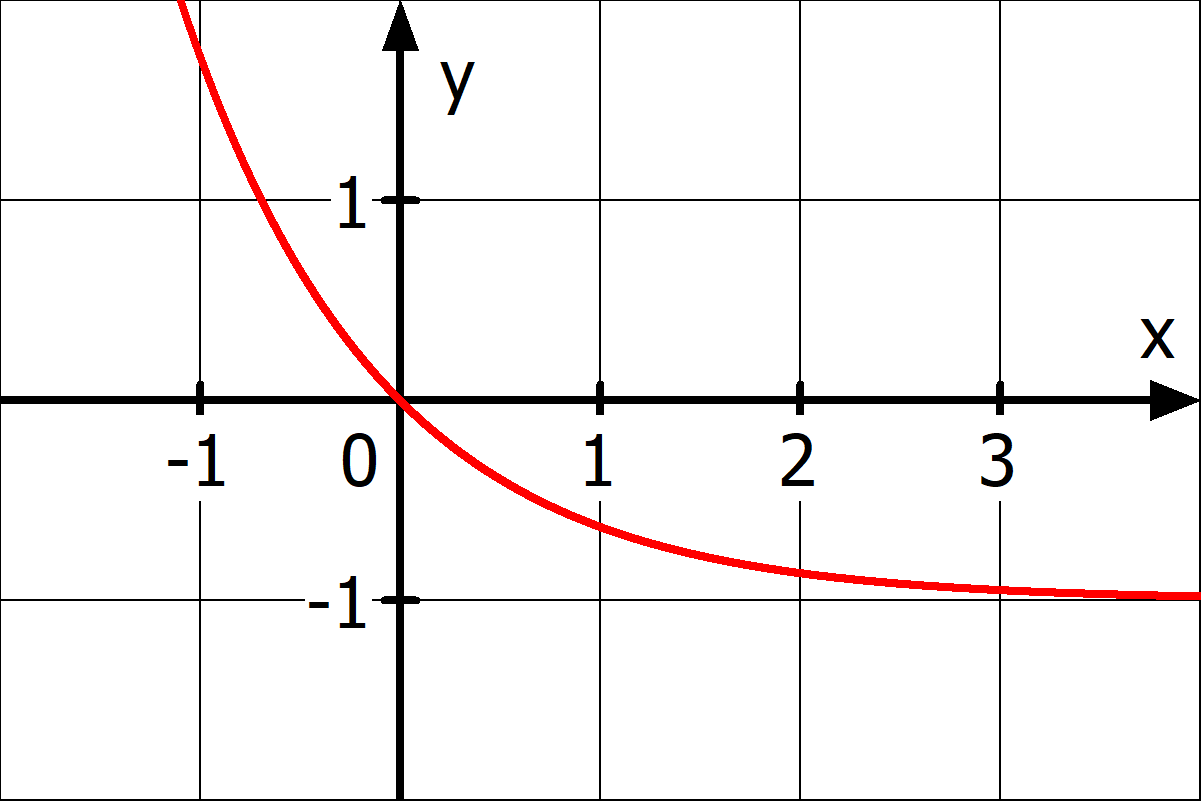
\includegraphics[width=\textwidth]{\ableitung/pics/monotonieBsp2.png}
	\end{minipage}}%
\end{minipage}

\bigskip

\begin{minipage}{\textwidth}
	\adjustbox{valign=t, padding=0ex 0ex 2ex 0ex}{\begin{minipage}{0.4\textwidth-2ex}
		\centering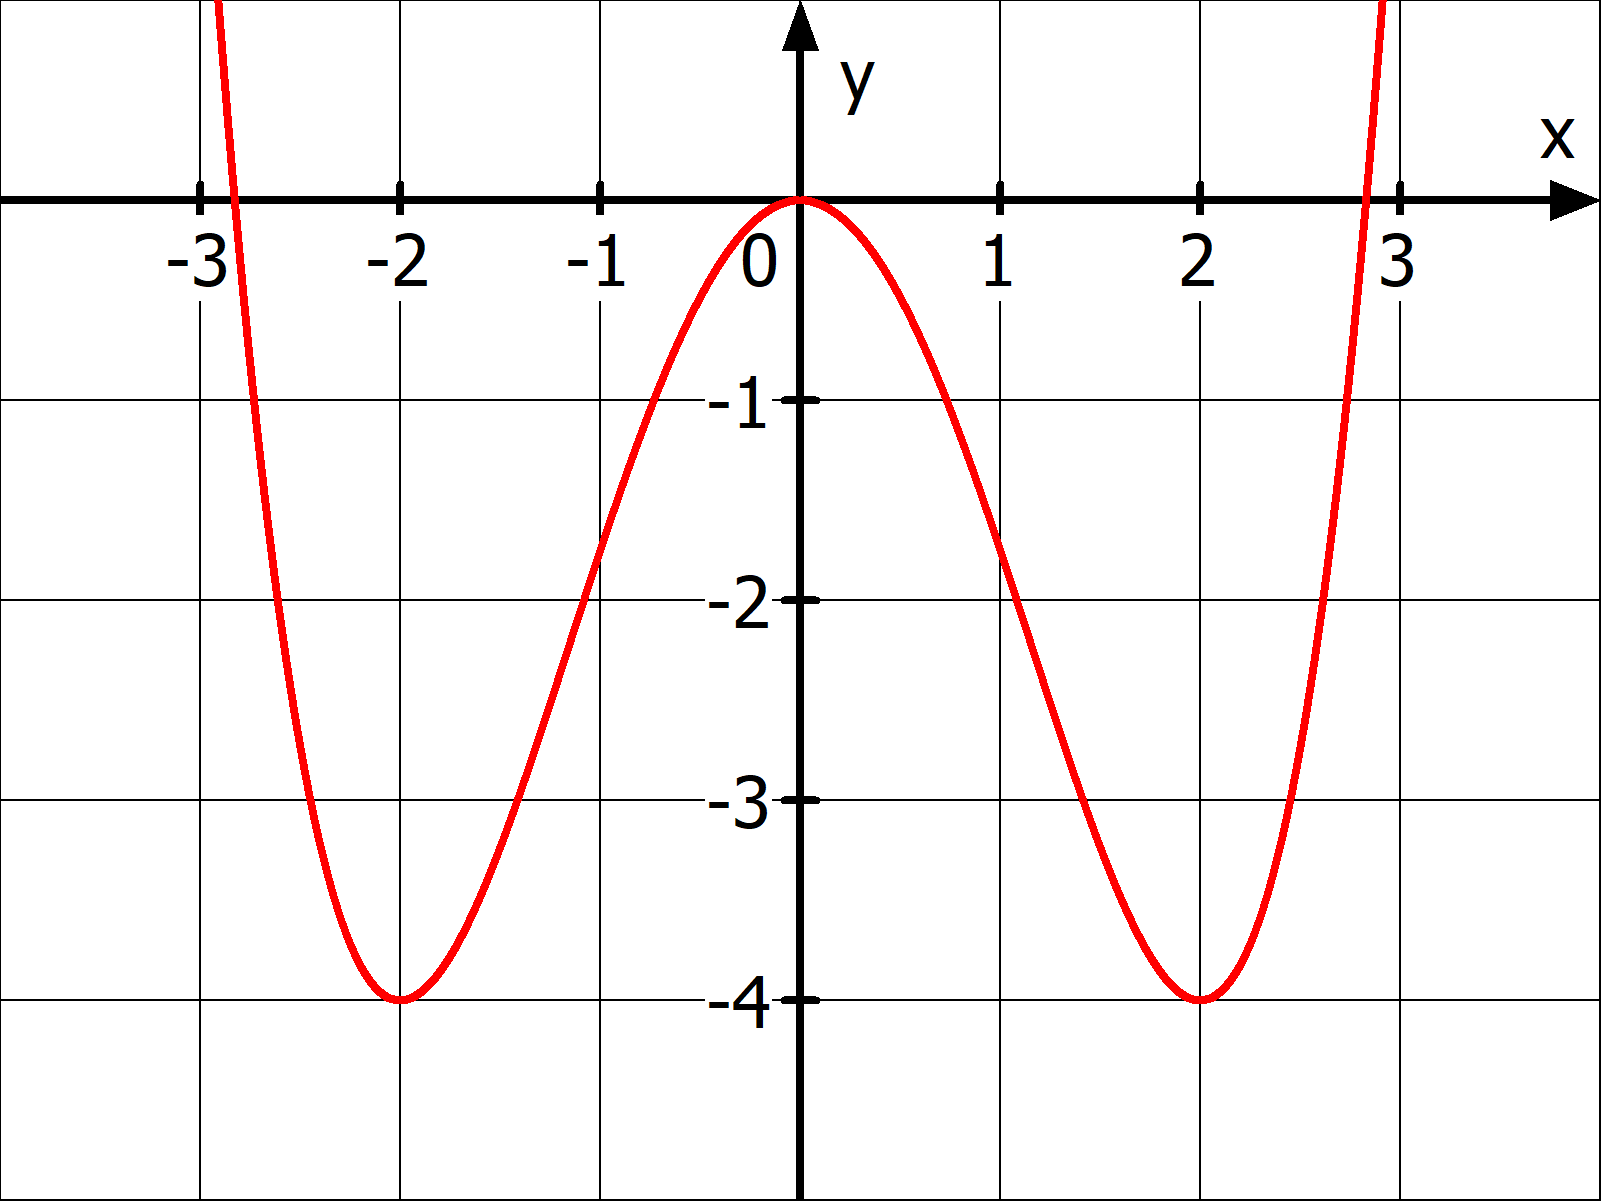
\includegraphics[width=\textwidth]{\ableitung/pics/monotonieBsp3.png}
	\end{minipage}}%
	\adjustbox{valign=t}{\begin{minipage}{0.6\textwidth}
		Monotonie kann auch für Intervalle definiert werden:

		Die Funktion \(f(x)=\frac{1}{4}x^4-2x^2\) hat folgende Monotonieintervalle:

		\textcolor{loes}{Auf den Intervallen \(]-\infty,\ -2]\) und \([0,\ 2]\) ist die Funktion monoton fallend.}

		\textcolor{loes}{Auf den Intervallen \([-2,\ 0]\) und \([2,\ \infty[\) ist die Funktion monoton steigend.}
	\end{minipage}}%
\end{minipage}

\bigskip

\textcolor{loes}{Hinweis: Wir unterscheiden nicht zwischen Monotonie und strenger Monotonie}
\newpage
%%%%%%%%%%%%%%%%%%%%%%%%%%%%%%%%%%%%%%%%%%%%%%%%%%%%%%%%%%%%%%%%%%%%%%%%%%%%%%%%%%%%%%%%%%%%%%%%%%%%%%%
\begin{Exercise}[title={\raggedright Bestimme die Monotonieintervalle.}, label=monotonieA1]

	\begin{minipage}{\textwidth}
		\adjustbox{valign=t, padding=0ex 0ex 0ex 0ex}{\begin{minipage}{\textwidth/\real{3}-2ex}
			\centering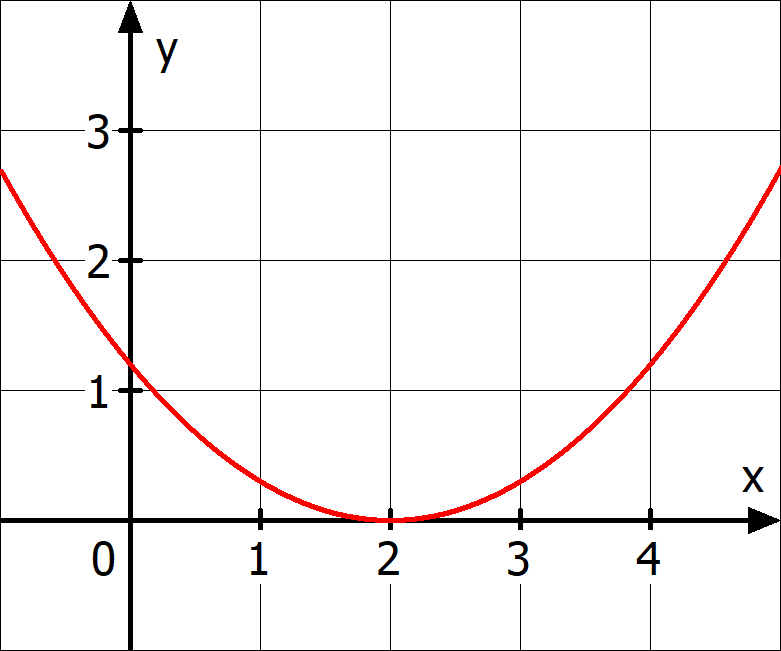
\includegraphics[width=\textwidth]{\ableitung/pics/monotonieIntervalle1.png}
		\end{minipage}}%
		\adjustbox{valign=t, padding=3ex 0ex 0ex 0ex}{\begin{minipage}{\textwidth/\real{3}-2ex}
			\centering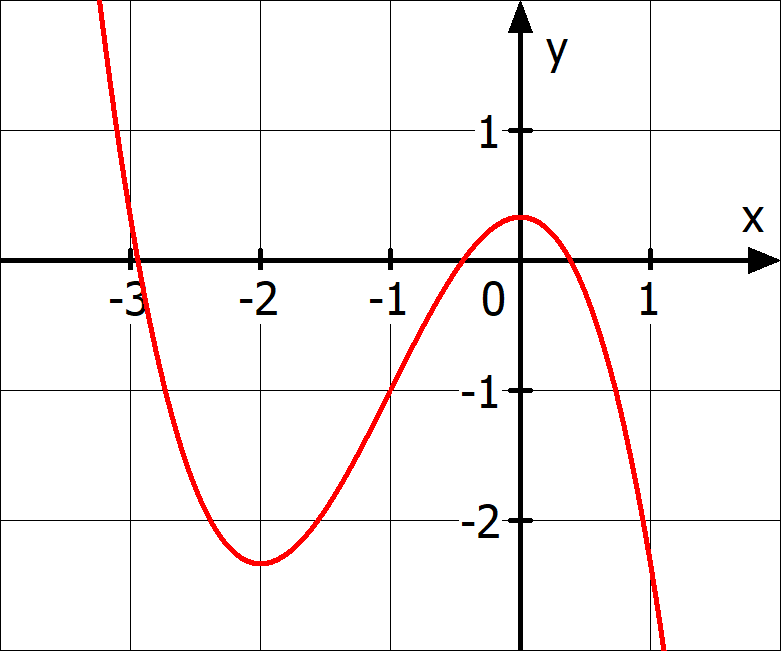
\includegraphics[width=\textwidth]{\ableitung/pics/monotonieIntervalle2.png}
		\end{minipage}}%
		\adjustbox{valign=t, padding=3ex 0ex 0ex 0ex}{\begin{minipage}{\textwidth/\real{3}-2ex}
			\centering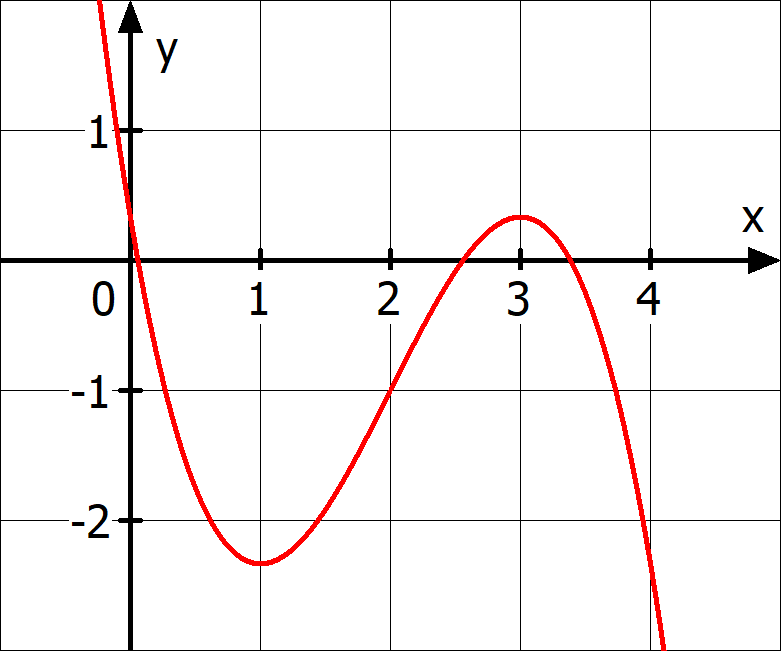
\includegraphics[width=\textwidth]{\ableitung/pics/monotonieIntervalle3.png}
		\end{minipage}}%
    \end{minipage}%

    \vspace{3ex}

    \begin{minipage}{\textwidth}
		\adjustbox{valign=t, padding=0ex 0ex 0ex 0ex}{\begin{minipage}{\textwidth/\real{3}-2ex}
			\centering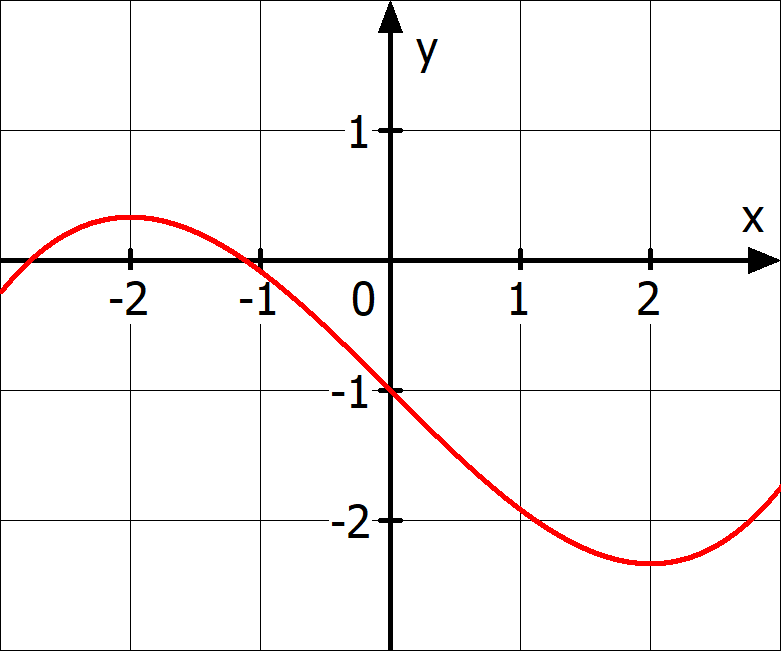
\includegraphics[width=\textwidth]{\ableitung/pics/monotonieIntervalle4.png}
		\end{minipage}}%
		\adjustbox{valign=t, padding=3ex 0ex 0ex 0ex}{\begin{minipage}{\textwidth/\real{3}-2ex}
			\centering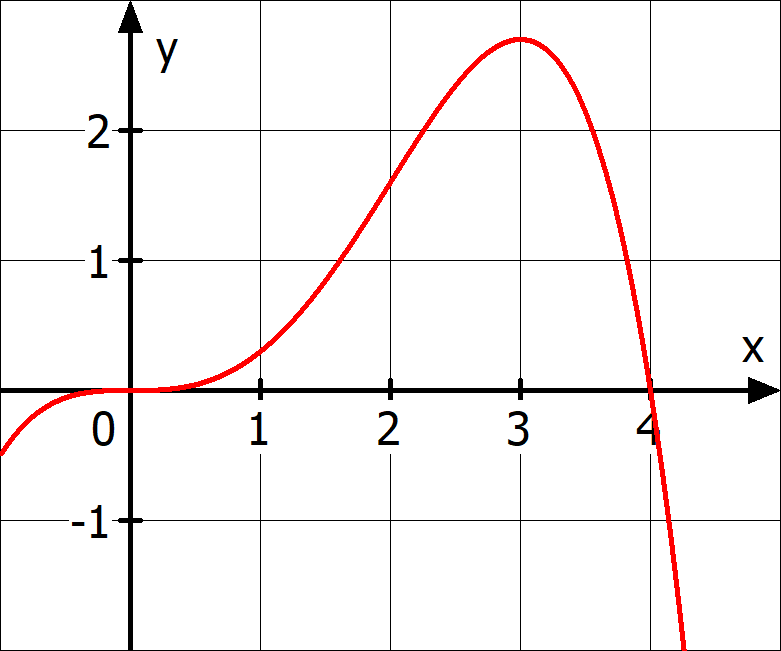
\includegraphics[width=\textwidth]{\ableitung/pics/monotonieIntervalle5.png}
		\end{minipage}}%
		\adjustbox{valign=t, padding=3ex 0ex 0ex 0ex}{\begin{minipage}{\textwidth/\real{3}-2ex}
			\centering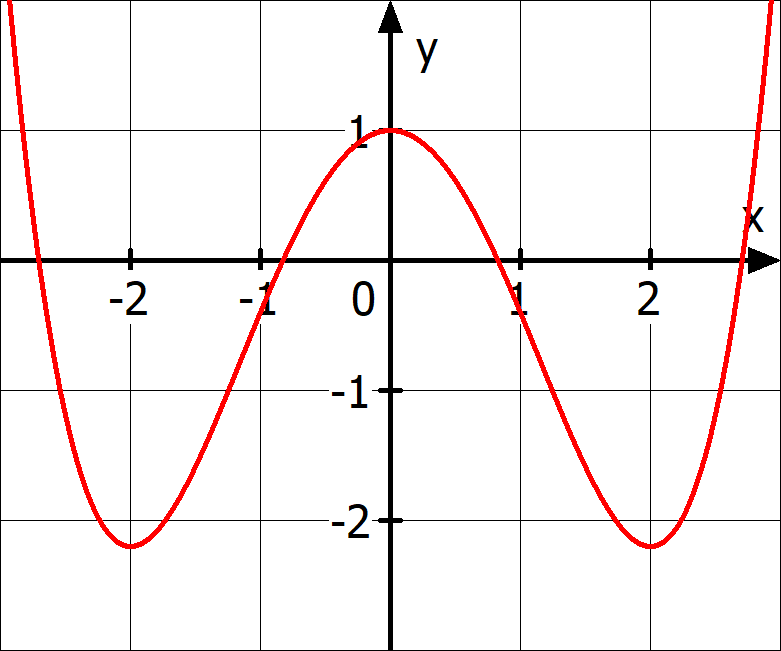
\includegraphics[width=\textwidth]{\ableitung/pics/monotonieIntervalle6.png}
		\end{minipage}}%
    \end{minipage}%

    \vspace{3ex}

    \begin{minipage}{\textwidth}
		\adjustbox{valign=t, padding=0ex 0ex 0ex 0ex}{\begin{minipage}{\textwidth/\real{3}-2ex}
			\centering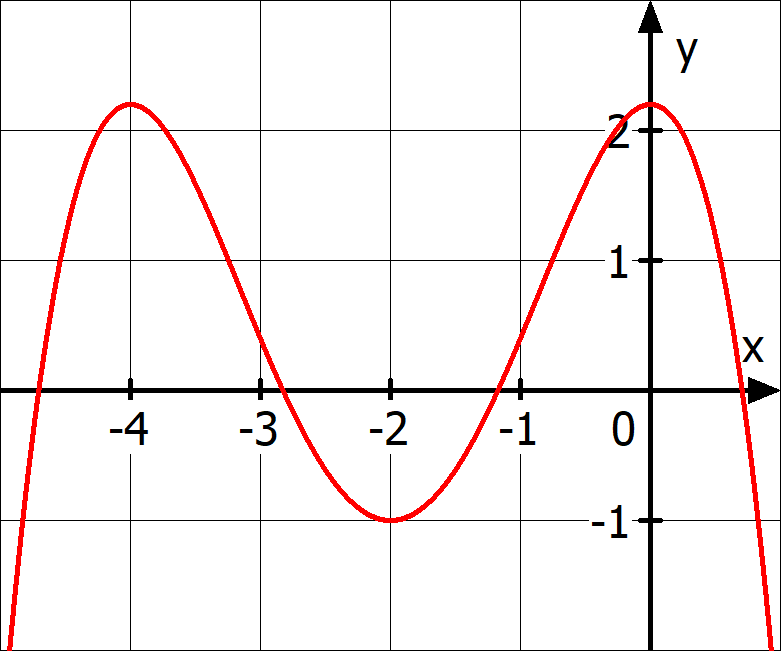
\includegraphics[width=\textwidth]{\ableitung/pics/monotonieIntervalle7.png}
		\end{minipage}}%
		\adjustbox{valign=t, padding=3ex 0ex 0ex 0ex}{\begin{minipage}{\textwidth/\real{3}-2ex}
			\centering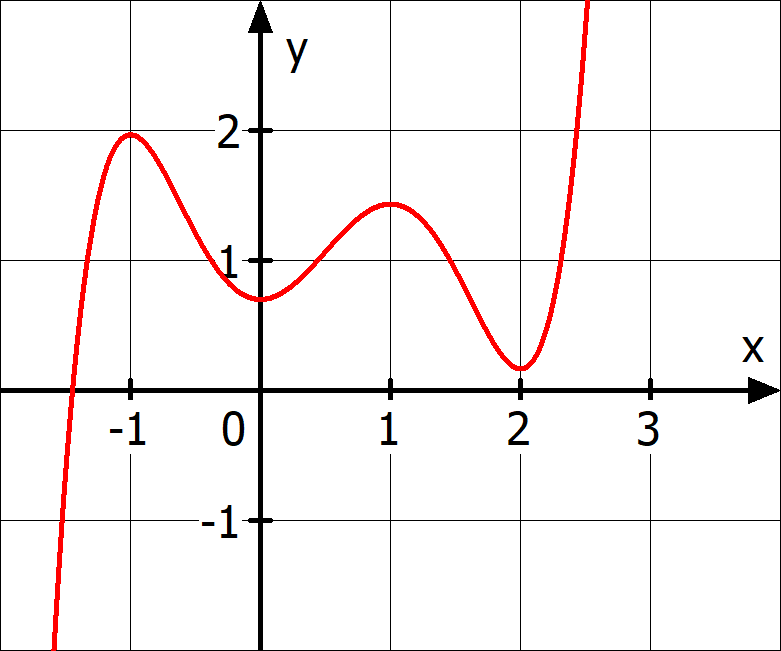
\includegraphics[width=\textwidth]{\ableitung/pics/monotonieIntervalle8.png}
		\end{minipage}}%
		\adjustbox{valign=t, padding=3ex 0ex 0ex 0ex}{\begin{minipage}{\textwidth/\real{3}-2ex}
			\centering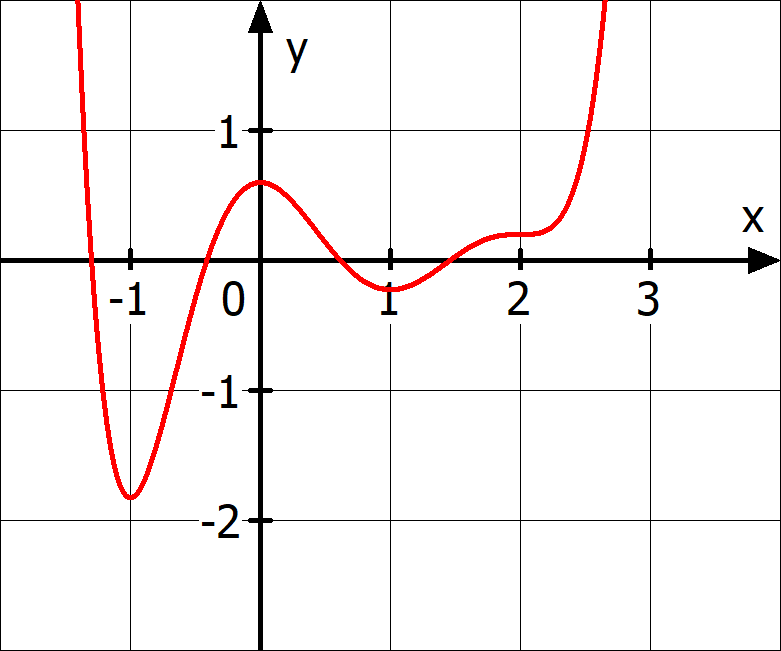
\includegraphics[width=\textwidth]{\ableitung/pics/monotonieIntervalle9.png}
		\end{minipage}}%
	\end{minipage}%
\end{Exercise}
%%%%%%%%%%%%%%%%%%%%%%%%%%%%%%%%%%%%%%%%%
\begin{Answer}[ref=monotonieA1]

	\begin{tabular}{p{.3\textwidth}|p{.3\textwidth}|p{.3\textwidth}}
		\hline
		Monoton fallend auf\newline \(]-\infty;2]\)\newline
		Monoton steigend auf\newline \([2;\infty[\)
		&
		Monoton fallend auf\newline \(]-\infty;-2]\) und \([0;\infty[\)\newline
		Monoton steigend auf\newline \([-2;0]\)
		&
		Monoton fallend auf\newline \(]-\infty;1]\) und \([3;\infty[\)\newline
		Monoton steigend auf\newline \([1;3]\)
		\\
		\hline
		Monoton fallend auf\newline \([-2;2]\)\newline
		Monoton steigend auf\newline \(]-\infty;-2]\) und \([2;\infty[\)
		&
		Monoton fallend auf\newline \([3;\infty[\)\newline
		Monoton steigend auf\newline \(]-\infty;3]\)
		&
		Monoton fallend auf\newline \(]-\infty;-2]\) und \([1;2]\)\newline
		Monoton steigend auf\newline \([-2;0]\) und \([2;\infty[\)
		\\
		\hline
		Monoton fallend auf\newline \([-4;-2]\) und \([0;\infty[\)\newline
		Monoton steigend auf\newline \(]-\infty;-4]\) und \([-2;0]\)
		&
		Monoton fallend auf\newline \([-1;0]\) und \([1;2]\)\newline
		Monoton steigend auf\newline \(]-\infty;-1]\), \([0;1]\) und \([1;\infty[\)
		&
		Monoton fallend auf\newline \(]-\infty;-1]\) und \([0;1]\)\newline
		Monoton steigend auf\newline \([-1;0]\) und \([1;\infty[\)
		\\
		\hline
	\end{tabular}
\end{Answer}